% Options for packages loaded elsewhere
\PassOptionsToPackage{unicode}{hyperref}
\PassOptionsToPackage{hyphens}{url}
\PassOptionsToPackage{dvipsnames,svgnames,x11names}{xcolor}
%
\documentclass[
  12pt,
]{report}

\usepackage{amsmath,amssymb}
\usepackage{iftex}
\ifPDFTeX
  \usepackage[T1]{fontenc}
  \usepackage[utf8]{inputenc}
  \usepackage{textcomp} % provide euro and other symbols
\else % if luatex or xetex
  \usepackage{unicode-math}
  \defaultfontfeatures{Scale=MatchLowercase}
  \defaultfontfeatures[\rmfamily]{Ligatures=TeX,Scale=1}
\fi
\usepackage[]{arial}
\ifPDFTeX\else  
    % xetex/luatex font selection
\fi
% Use upquote if available, for straight quotes in verbatim environments
\IfFileExists{upquote.sty}{\usepackage{upquote}}{}
\IfFileExists{microtype.sty}{% use microtype if available
  \usepackage[]{microtype}
  \UseMicrotypeSet[protrusion]{basicmath} % disable protrusion for tt fonts
}{}
\makeatletter
\@ifundefined{KOMAClassName}{% if non-KOMA class
  \IfFileExists{parskip.sty}{%
    \usepackage{parskip}
  }{% else
    \setlength{\parindent}{0pt}
    \setlength{\parskip}{6pt plus 2pt minus 1pt}}
}{% if KOMA class
  \KOMAoptions{parskip=half}}
\makeatother
\usepackage{xcolor}
\usepackage[margin=1in]{geometry}
\setlength{\emergencystretch}{3em} % prevent overfull lines
\setcounter{secnumdepth}{-\maxdimen} % remove section numbering
% Make \paragraph and \subparagraph free-standing
\makeatletter
\ifx\paragraph\undefined\else
  \let\oldparagraph\paragraph
  \renewcommand{\paragraph}{
    \@ifstar
      \xxxParagraphStar
      \xxxParagraphNoStar
  }
  \newcommand{\xxxParagraphStar}[1]{\oldparagraph*{#1}\mbox{}}
  \newcommand{\xxxParagraphNoStar}[1]{\oldparagraph{#1}\mbox{}}
\fi
\ifx\subparagraph\undefined\else
  \let\oldsubparagraph\subparagraph
  \renewcommand{\subparagraph}{
    \@ifstar
      \xxxSubParagraphStar
      \xxxSubParagraphNoStar
  }
  \newcommand{\xxxSubParagraphStar}[1]{\oldsubparagraph*{#1}\mbox{}}
  \newcommand{\xxxSubParagraphNoStar}[1]{\oldsubparagraph{#1}\mbox{}}
\fi
\makeatother

\usepackage{color}
\usepackage{fancyvrb}
\newcommand{\VerbBar}{|}
\newcommand{\VERB}{\Verb[commandchars=\\\{\}]}
\DefineVerbatimEnvironment{Highlighting}{Verbatim}{commandchars=\\\{\}}
% Add ',fontsize=\small' for more characters per line
\usepackage{framed}
\definecolor{shadecolor}{RGB}{241,243,245}
\newenvironment{Shaded}{\begin{snugshade}}{\end{snugshade}}
\newcommand{\AlertTok}[1]{\textcolor[rgb]{0.68,0.00,0.00}{#1}}
\newcommand{\AnnotationTok}[1]{\textcolor[rgb]{0.37,0.37,0.37}{#1}}
\newcommand{\AttributeTok}[1]{\textcolor[rgb]{0.40,0.45,0.13}{#1}}
\newcommand{\BaseNTok}[1]{\textcolor[rgb]{0.68,0.00,0.00}{#1}}
\newcommand{\BuiltInTok}[1]{\textcolor[rgb]{0.00,0.23,0.31}{#1}}
\newcommand{\CharTok}[1]{\textcolor[rgb]{0.13,0.47,0.30}{#1}}
\newcommand{\CommentTok}[1]{\textcolor[rgb]{0.37,0.37,0.37}{#1}}
\newcommand{\CommentVarTok}[1]{\textcolor[rgb]{0.37,0.37,0.37}{\textit{#1}}}
\newcommand{\ConstantTok}[1]{\textcolor[rgb]{0.56,0.35,0.01}{#1}}
\newcommand{\ControlFlowTok}[1]{\textcolor[rgb]{0.00,0.23,0.31}{\textbf{#1}}}
\newcommand{\DataTypeTok}[1]{\textcolor[rgb]{0.68,0.00,0.00}{#1}}
\newcommand{\DecValTok}[1]{\textcolor[rgb]{0.68,0.00,0.00}{#1}}
\newcommand{\DocumentationTok}[1]{\textcolor[rgb]{0.37,0.37,0.37}{\textit{#1}}}
\newcommand{\ErrorTok}[1]{\textcolor[rgb]{0.68,0.00,0.00}{#1}}
\newcommand{\ExtensionTok}[1]{\textcolor[rgb]{0.00,0.23,0.31}{#1}}
\newcommand{\FloatTok}[1]{\textcolor[rgb]{0.68,0.00,0.00}{#1}}
\newcommand{\FunctionTok}[1]{\textcolor[rgb]{0.28,0.35,0.67}{#1}}
\newcommand{\ImportTok}[1]{\textcolor[rgb]{0.00,0.46,0.62}{#1}}
\newcommand{\InformationTok}[1]{\textcolor[rgb]{0.37,0.37,0.37}{#1}}
\newcommand{\KeywordTok}[1]{\textcolor[rgb]{0.00,0.23,0.31}{\textbf{#1}}}
\newcommand{\NormalTok}[1]{\textcolor[rgb]{0.00,0.23,0.31}{#1}}
\newcommand{\OperatorTok}[1]{\textcolor[rgb]{0.37,0.37,0.37}{#1}}
\newcommand{\OtherTok}[1]{\textcolor[rgb]{0.00,0.23,0.31}{#1}}
\newcommand{\PreprocessorTok}[1]{\textcolor[rgb]{0.68,0.00,0.00}{#1}}
\newcommand{\RegionMarkerTok}[1]{\textcolor[rgb]{0.00,0.23,0.31}{#1}}
\newcommand{\SpecialCharTok}[1]{\textcolor[rgb]{0.37,0.37,0.37}{#1}}
\newcommand{\SpecialStringTok}[1]{\textcolor[rgb]{0.13,0.47,0.30}{#1}}
\newcommand{\StringTok}[1]{\textcolor[rgb]{0.13,0.47,0.30}{#1}}
\newcommand{\VariableTok}[1]{\textcolor[rgb]{0.07,0.07,0.07}{#1}}
\newcommand{\VerbatimStringTok}[1]{\textcolor[rgb]{0.13,0.47,0.30}{#1}}
\newcommand{\WarningTok}[1]{\textcolor[rgb]{0.37,0.37,0.37}{\textit{#1}}}

\providecommand{\tightlist}{%
  \setlength{\itemsep}{0pt}\setlength{\parskip}{0pt}}\usepackage{longtable,booktabs,array}
\usepackage{calc} % for calculating minipage widths
% Correct order of tables after \paragraph or \subparagraph
\usepackage{etoolbox}
\makeatletter
\patchcmd\longtable{\par}{\if@noskipsec\mbox{}\fi\par}{}{}
\makeatother
% Allow footnotes in longtable head/foot
\IfFileExists{footnotehyper.sty}{\usepackage{footnotehyper}}{\usepackage{footnote}}
\makesavenoteenv{longtable}
\usepackage{graphicx}
\makeatletter
\def\maxwidth{\ifdim\Gin@nat@width>\linewidth\linewidth\else\Gin@nat@width\fi}
\def\maxheight{\ifdim\Gin@nat@height>\textheight\textheight\else\Gin@nat@height\fi}
\makeatother
% Scale images if necessary, so that they will not overflow the page
% margins by default, and it is still possible to overwrite the defaults
% using explicit options in \includegraphics[width, height, ...]{}
\setkeys{Gin}{width=\maxwidth,height=\maxheight,keepaspectratio}
% Set default figure placement to htbp
\makeatletter
\def\fps@figure{htbp}
\makeatother

\makeatletter
\@ifpackageloaded{caption}{}{\usepackage{caption}}
\AtBeginDocument{%
\ifdefined\contentsname
  \renewcommand*\contentsname{Índice}
\else
  \newcommand\contentsname{Índice}
\fi
\ifdefined\listfigurename
  \renewcommand*\listfigurename{Lista de Figuras}
\else
  \newcommand\listfigurename{Lista de Figuras}
\fi
\ifdefined\listtablename
  \renewcommand*\listtablename{Lista de Tabelas}
\else
  \newcommand\listtablename{Lista de Tabelas}
\fi
\ifdefined\figurename
  \renewcommand*\figurename{Figura}
\else
  \newcommand\figurename{Figura}
\fi
\ifdefined\tablename
  \renewcommand*\tablename{Tabela}
\else
  \newcommand\tablename{Tabela}
\fi
}
\@ifpackageloaded{float}{}{\usepackage{float}}
\floatstyle{ruled}
\@ifundefined{c@chapter}{\newfloat{codelisting}{h}{lop}}{\newfloat{codelisting}{h}{lop}[chapter]}
\floatname{codelisting}{Listagem}
\newcommand*\listoflistings{\listof{codelisting}{Lista de Listagens}}
\makeatother
\makeatletter
\makeatother
\makeatletter
\@ifpackageloaded{caption}{}{\usepackage{caption}}
\@ifpackageloaded{subcaption}{}{\usepackage{subcaption}}
\makeatother

\ifLuaTeX
\usepackage[bidi=basic]{babel}
\else
\usepackage[bidi=default]{babel}
\fi
\babelprovide[main,import]{brazilian}
% get rid of language-specific shorthands (see #6817):
\let\LanguageShortHands\languageshorthands
\def\languageshorthands#1{}
\ifLuaTeX
  \usepackage{selnolig}  % disable illegal ligatures
\fi
\usepackage{bookmark}

\IfFileExists{xurl.sty}{\usepackage{xurl}}{} % add URL line breaks if available
\urlstyle{same} % disable monospaced font for URLs
\hypersetup{
  pdftitle={ElasticSearch e linguagem R para análise de violência política na plataforma Telegram},
  pdfauthor={Ruan Arthur Lima Santos},
  pdflang={pt-BR},
  colorlinks=true,
  linkcolor={blue},
  filecolor={Maroon},
  citecolor={Blue},
  urlcolor={Blue},
  pdfcreator={LaTeX via pandoc}}


\title{ElasticSearch e linguagem R para análise de violência política na
plataforma Telegram}
\usepackage{etoolbox}
\makeatletter
\providecommand{\subtitle}[1]{% add subtitle to \maketitle
  \apptocmd{\@title}{\par {\large #1 \par}}{}{}
}
\makeatother
\subtitle{Guilherme Boulos em \texttt{chats} do \texttt{Telegram}}
\author{Ruan Arthur Lima Santos}
\date{}

\begin{document}
\maketitle

\renewcommand*\contentsname{Índice}
{
\hypersetup{linkcolor=}
\setcounter{tocdepth}{2}
\tableofcontents
}

\begin{center}\rule{0.5\linewidth}{0.5pt}\end{center}

\chapter{Critérios de busca}\label{crituxe9rios-de-busca}

\begin{quote}
\textbf{\emph{query:}}
\texttt{all\_text:\ "guilherme\ boulos"\ or\ boulos}

\emph{período: Set 9, 2023, 00:00h \& Nov 3, 2024 23:59h}
\end{quote}

\begin{center}\rule{0.5\linewidth}{0.5pt}\end{center}

\chapter{Análise de sentimento com
R}\label{anuxe1lise-de-sentimento-com-r}

\section{Bibliotecas}\label{bibliotecas}

\begin{Shaded}
\begin{Highlighting}[]
\FunctionTok{library}\NormalTok{(syuzhet)}
\FunctionTok{library}\NormalTok{(RColorBrewer)}
\FunctionTok{library}\NormalTok{(wordcloud)}
\FunctionTok{library}\NormalTok{(tm)}
\FunctionTok{library}\NormalTok{(tidyverse)}
\FunctionTok{library}\NormalTok{(extrafont)}
\end{Highlighting}
\end{Shaded}

\section{\texorpdfstring{Criando objeto
\texttt{mensagens\_brutas}}{Criando objeto mensagens\_brutas}}\label{criando-objeto-mensagens_brutas}

\begin{Shaded}
\begin{Highlighting}[]
\NormalTok{mensagens\_brutas }\OtherTok{\textless{}{-}} \FunctionTok{read.csv}\NormalTok{(}\AttributeTok{file =} \StringTok{"dados/mensagens\_boulos.csv"}\NormalTok{)}
\end{Highlighting}
\end{Shaded}

\section{Manipulando a base}\label{manipulando-a-base}

\begin{Shaded}
\begin{Highlighting}[]
\NormalTok{mensagens\_brutas }\OtherTok{\textless{}{-}}\NormalTok{ mensagens\_brutas }\SpecialCharTok{|\textgreater{}} 
  \FunctionTok{rename}\NormalTok{(}\AttributeTok{mensagens =}\NormalTok{ Top.values.of.all\_text.keyword,}
         \AttributeTok{compartilhamentos =}\NormalTok{ Count.of.records) }\SpecialCharTok{|\textgreater{}} 
  \FunctionTok{filter}\NormalTok{(mensagens }\SpecialCharTok{!=} \StringTok{"Other"}\NormalTok{) }\SpecialCharTok{|\textgreater{}} 
  \FunctionTok{mutate}\NormalTok{(}
    \AttributeTok{compartilhamentos =} \FunctionTok{as.integer}\NormalTok{(compartilhamentos)}
\NormalTok{  )}

\NormalTok{mensagens\_brutas }\OtherTok{\textless{}{-}}\NormalTok{ mensagens\_brutas }\SpecialCharTok{|\textgreater{}}
  \FunctionTok{mutate}\NormalTok{(}
    \AttributeTok{mensagens =}\NormalTok{ mensagens }\SpecialCharTok{|\textgreater{}} \FunctionTok{str\_trim}\NormalTok{(}\AttributeTok{side =} \StringTok{"both"}\NormalTok{)}
\NormalTok{  )}
\end{Highlighting}
\end{Shaded}

\section{\texorpdfstring{Obter
\texttt{tokens}}{Obter tokens}}\label{obter-tokens}

\begin{Shaded}
\begin{Highlighting}[]
\NormalTok{texto\_palavras }\OtherTok{\textless{}{-}} \FunctionTok{get\_tokens}\NormalTok{(}\AttributeTok{text\_of\_file =}\NormalTok{ mensagens\_brutas}\SpecialCharTok{$}\NormalTok{mensagens) }\CommentTok{\# pegando os tokens}

\NormalTok{texto\_sentencas }\OtherTok{\textless{}{-}} \FunctionTok{get\_sentences}\NormalTok{(}\AttributeTok{text\_of\_file =}\NormalTok{ mensagens\_brutas}\SpecialCharTok{$}\NormalTok{mensagens) }\CommentTok{\# pegando as sentenças}
\end{Highlighting}
\end{Shaded}

\section{Palavras mais repetidas / Dicionário próprio (tira
samerda)}\label{palavras-mais-repetidas-dicionuxe1rio-pruxf3prio-tira-samerda}

\begin{Shaded}
\begin{Highlighting}[]
\NormalTok{mensagem\_palavras }\OtherTok{\textless{}{-}} \FunctionTok{data.frame}\NormalTok{(}
  \AttributeTok{palavras =} \FunctionTok{scan}\NormalTok{(}\AttributeTok{text =}\NormalTok{ mensagens\_brutas}\SpecialCharTok{$}\NormalTok{mensagens,}
                          \AttributeTok{what =} \FunctionTok{character}\NormalTok{(),}
                          \AttributeTok{allowEscapes =}\NormalTok{ T,}
                          \AttributeTok{fileEncoding =} \StringTok{"UTF{-}8"}\NormalTok{)}

\NormalTok{)}

\NormalTok{termos }\OtherTok{\textless{}{-}} \FunctionTok{c}\NormalTok{(}\StringTok{"comunista"}\NormalTok{, }\StringTok{"esquerda"}\NormalTok{, }\StringTok{"comuna"}\NormalTok{, }\StringTok{"esquerdalha"}\NormalTok{, }\StringTok{"esquerdopata"}\NormalTok{, }\StringTok{"ladrao"}\NormalTok{, }\StringTok{"roubo"}\NormalTok{, }\StringTok{"invasao"}\NormalTok{, }\StringTok{"drogas"}\NormalTok{, }\StringTok{"maconha"}\NormalTok{, }\StringTok{"mst"}\NormalTok{)}

\NormalTok{dicionario }\OtherTok{\textless{}{-}} \FunctionTok{tibble}\NormalTok{(}
  \AttributeTok{palavras =}\NormalTok{ termos,}
  \AttributeTok{anger =} \FunctionTok{rep}\NormalTok{(}\DecValTok{1}\NormalTok{, }\FunctionTok{length}\NormalTok{(termos))}
\NormalTok{)}

\NormalTok{palavras\_mais\_repetidas }\OtherTok{\textless{}{-}}\NormalTok{ mensagem\_palavras }\SpecialCharTok{|\textgreater{}} 
  \FunctionTok{count}\NormalTok{(palavras, }\AttributeTok{sort =}\NormalTok{ T)}

\NormalTok{filtro }\OtherTok{\textless{}{-}} \FunctionTok{c}\NormalTok{( }\StringTok{"boulos"}\NormalTok{, }\StringTok{"boulo"}\NormalTok{, }\StringTok{"guilherme"}\NormalTok{, }\StringTok{"a"}\NormalTok{, }\StringTok{"o"}\NormalTok{, }\StringTok{"e"}\NormalTok{, }\StringTok{"ante"}\NormalTok{, }\StringTok{"até"}\NormalTok{, }\StringTok{"com"}\NormalTok{, }\StringTok{"contra"}\NormalTok{, }\StringTok{"de"}\NormalTok{, }\StringTok{"desde"}\NormalTok{, }\StringTok{"em"}\NormalTok{, }\StringTok{"entre"}\NormalTok{, }\StringTok{"para"}\NormalTok{, }\StringTok{"pra"}\NormalTok{, }\StringTok{"perante"}\NormalTok{, }\StringTok{"por"}\NormalTok{, }\StringTok{"sem"}\NormalTok{, }\StringTok{"sobre"}\NormalTok{, }\StringTok{"trás"}\NormalTok{, }\StringTok{"com"}\NormalTok{, }\StringTok{"num"}\NormalTok{, }\StringTok{"numa"}\NormalTok{, }\StringTok{"aquilo"}\NormalTok{, }\StringTok{"aquele"}\NormalTok{, }\StringTok{"aquela"}\NormalTok{, }\StringTok{"que"}\NormalTok{, }\StringTok{"do"}\NormalTok{, }\StringTok{"é"}\NormalTok{, }\StringTok{"no"}\NormalTok{, }\StringTok{"na"}\NormalTok{, }\StringTok{"da"}\NormalTok{)}

\NormalTok{palavras\_mais\_repetidas }\OtherTok{\textless{}{-}}\NormalTok{ palavras\_mais\_repetidas }\SpecialCharTok{|\textgreater{}} 
  \FunctionTok{filter}\NormalTok{(}\SpecialCharTok{!}\FunctionTok{str\_to\_lower}\NormalTok{(palavras) }\SpecialCharTok{\%in\%}\NormalTok{ filtro)}
\end{Highlighting}
\end{Shaded}

\section{Análise de sentimento}\label{anuxe1lise-de-sentimento}

\begin{Shaded}
\begin{Highlighting}[]
\NormalTok{sentimentos\_tokens }\OtherTok{\textless{}{-}} \FunctionTok{get\_nrc\_sentiment}\NormalTok{(}\AttributeTok{char\_v =}\NormalTok{ texto\_palavras, }\AttributeTok{language =} \StringTok{"portuguese"}\NormalTok{)}

\NormalTok{sentimentos\_sentencas }\OtherTok{\textless{}{-}} \FunctionTok{get\_nrc\_sentiment}\NormalTok{(}\AttributeTok{char\_v =}\NormalTok{ texto\_sentencas, }\AttributeTok{language =} \StringTok{"portuguese"}\NormalTok{)}


\FunctionTok{summary}\NormalTok{(sentimentos\_sentencas)}
\end{Highlighting}
\end{Shaded}

\begin{verbatim}
     anger       anticipation       disgust            fear       
 Min.   :0.00   Min.   :0.0000   Min.   :0.0000   Min.   :0.0000  
 1st Qu.:0.00   1st Qu.:0.0000   1st Qu.:0.0000   1st Qu.:0.0000  
 Median :0.00   Median :0.0000   Median :0.0000   Median :0.0000  
 Mean   :0.22   Mean   :0.1599   Mean   :0.1377   Mean   :0.2019  
 3rd Qu.:0.00   3rd Qu.:0.0000   3rd Qu.:0.0000   3rd Qu.:0.0000  
 Max.   :3.00   Max.   :4.0000   Max.   :4.0000   Max.   :4.0000  
      joy            sadness          surprise          trust      
 Min.   :0.0000   Min.   :0.0000   Min.   :0.0000   Min.   :0.000  
 1st Qu.:0.0000   1st Qu.:0.0000   1st Qu.:0.0000   1st Qu.:0.000  
 Median :0.0000   Median :0.0000   Median :0.0000   Median :0.000  
 Mean   :0.1278   Mean   :0.2106   Mean   :0.1109   Mean   :0.248  
 3rd Qu.:0.0000   3rd Qu.:0.0000   3rd Qu.:0.0000   3rd Qu.:0.000  
 Max.   :5.0000   Max.   :4.0000   Max.   :3.0000   Max.   :4.000  
    negative         positive     
 Min.   :0.0000   Min.   :0.0000  
 1st Qu.:0.0000   1st Qu.:0.0000  
 Median :0.0000   Median :0.0000  
 Mean   :0.4947   Mean   :0.5519  
 3rd Qu.:1.0000   3rd Qu.:1.0000  
 Max.   :7.0000   Max.   :5.0000  
\end{verbatim}

\subsection{Gráfico de sentimentos com
sentenças}\label{gruxe1fico-de-sentimentos-com-sentenuxe7as}

\subsubsection{Manipulando os dados}\label{manipulando-os-dados}

\begin{Shaded}
\begin{Highlighting}[]
\CommentTok{\# Transformando os sentimentos em proporções}

\NormalTok{sentimentos\_sentencas\_prop }\OtherTok{\textless{}{-}} \FunctionTok{as.data.frame}\NormalTok{(}\FunctionTok{colSums}\NormalTok{(}\FunctionTok{prop.table}\NormalTok{(sentimentos\_sentencas))) }\CommentTok{\# criando o dataframe}

\FunctionTok{colnames}\NormalTok{(sentimentos\_sentencas\_prop) }\OtherTok{\textless{}{-}} \StringTok{"Proporção"} \CommentTok{\# Renomeando a coluna}

\NormalTok{sentimentos\_sentencas\_prop}\SpecialCharTok{$}\NormalTok{Emoções }\OtherTok{\textless{}{-}} \FunctionTok{rownames}\NormalTok{(sentimentos\_sentencas\_prop) }\CommentTok{\# Criando nova coluna "Emoções"}

\FunctionTok{rownames}\NormalTok{(sentimentos\_sentencas\_prop) }\OtherTok{\textless{}{-}} \ConstantTok{NULL} \CommentTok{\# Resetando o index}

\NormalTok{pn\_sentencas }\OtherTok{\textless{}{-}}\NormalTok{ sentimentos\_sentencas\_prop }\SpecialCharTok{|\textgreater{}} 
  \FunctionTok{filter}\NormalTok{(Emoções }\SpecialCharTok{==} \StringTok{"negative"} \SpecialCharTok{|}\NormalTok{ Emoções }\SpecialCharTok{==} \StringTok{"positive"}\NormalTok{)}\SpecialCharTok{|\textgreater{}} \CommentTok{\# Selecionando apenas os sentimentos}
  \FunctionTok{mutate}\NormalTok{(}
    \AttributeTok{Sentimentos =}\NormalTok{ Emoções }\SpecialCharTok{|\textgreater{}} \FunctionTok{recode}\NormalTok{(}\StringTok{"positive"} \OtherTok{=} \StringTok{"Positivo"}\NormalTok{,}
                                    \StringTok{"negative"} \OtherTok{=} \StringTok{"Negativo"}\NormalTok{)}
\NormalTok{  ) }\SpecialCharTok{|\textgreater{}} 
  \FunctionTok{select}\NormalTok{(}\SpecialCharTok{{-}}\NormalTok{Emoções)}

\NormalTok{sentimentos\_sentencas\_prop }\OtherTok{\textless{}{-}}\NormalTok{ sentimentos\_sentencas\_prop }\SpecialCharTok{|\textgreater{}}
  \FunctionTok{filter}\NormalTok{(Emoções }\SpecialCharTok{!=} \StringTok{"negative"} \SpecialCharTok{\&}\NormalTok{ Emoções }\SpecialCharTok{!=} \StringTok{"positive"}\NormalTok{) }\SpecialCharTok{|\textgreater{}} \CommentTok{\# Retirando apenas os sentimentos}
  \FunctionTok{mutate}\NormalTok{(Emoções }\OtherTok{=} \FunctionTok{recode}\NormalTok{( }\CommentTok{\# renomeando as emoções}
\NormalTok{    Emoções,}
    \StringTok{"anger"} \OtherTok{=} \StringTok{"Raiva"}\NormalTok{,}
    \StringTok{"anticipation"} \OtherTok{=} \StringTok{"Antecipação"}\NormalTok{,}
    \StringTok{"disgust"} \OtherTok{=} \StringTok{"Nojo"}\NormalTok{,}
    \StringTok{"fear"} \OtherTok{=} \StringTok{"Medo"}\NormalTok{,}
    \StringTok{"joy"} \OtherTok{=} \StringTok{"Alegria"}\NormalTok{,}
    \StringTok{"sadness"} \OtherTok{=} \StringTok{"Tristeza"}\NormalTok{,}
    \StringTok{"surprise"} \OtherTok{=} \StringTok{"Surpresa"}\NormalTok{,}
    \StringTok{"trust"} \OtherTok{=} \StringTok{"Confiança"}
\NormalTok{  ))}
\end{Highlighting}
\end{Shaded}

\subsubsection{Produzindo o gráfico}\label{produzindo-o-gruxe1fico}

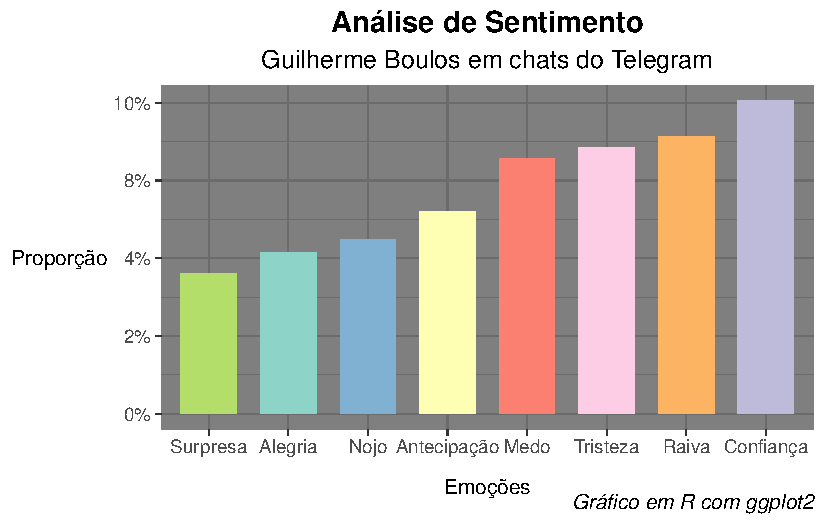
\includegraphics{boulos_files/figure-pdf/unnamed-chunk-8-1.pdf}

Nem falarei d'\texttt{Alegria}, me incomoda mais pensar em como diabos
\texttt{Confiança} alcançou um valor tão alto visto que extraímos
mensagens de \texttt{chats} de extrema-direita sobre \emph{Guilherme
Boulos?} Veremos:

\subsection{Nuvem de palavras}\label{nuvem-de-palavras}

\begin{Shaded}
\begin{Highlighting}[]
\NormalTok{palavras\_raiva }\OtherTok{\textless{}{-}}\NormalTok{ texto\_palavras[sentimentos\_tokens}\SpecialCharTok{$}\NormalTok{anger }\SpecialCharTok{\textgreater{}} \DecValTok{0}\NormalTok{]}

\NormalTok{tabela\_raiva }\OtherTok{\textless{}{-}}\NormalTok{ palavras\_raiva }\SpecialCharTok{|\textgreater{}} 
  \FunctionTok{table}\NormalTok{() }\SpecialCharTok{|\textgreater{}} \FunctionTok{sort}\NormalTok{(}\AttributeTok{decreasing =}\NormalTok{ T) }\SpecialCharTok{|\textgreater{}} \FunctionTok{head}\NormalTok{(}\DecValTok{10}\NormalTok{)}
  
\NormalTok{palavras\_confianca }\OtherTok{\textless{}{-}}\NormalTok{ texto\_palavras[sentimentos\_tokens}\SpecialCharTok{$}\NormalTok{trust }\SpecialCharTok{\textgreater{}} \DecValTok{0}\NormalTok{]}

\NormalTok{tabela\_confianca }\OtherTok{\textless{}{-}}\NormalTok{ palavras\_confianca }\SpecialCharTok{|\textgreater{}} 
  \FunctionTok{table}\NormalTok{() }\SpecialCharTok{|\textgreater{}} \FunctionTok{sort}\NormalTok{(}\AttributeTok{decreasing =}\NormalTok{ T) }\SpecialCharTok{|\textgreater{}} \FunctionTok{head}\NormalTok{(}\DecValTok{10}\NormalTok{)}

\NormalTok{nuvem\_emocoes\_vetor }\OtherTok{\textless{}{-}} \FunctionTok{c}\NormalTok{(}
\FunctionTok{paste}\NormalTok{(texto\_palavras[sentimentos\_tokens}\SpecialCharTok{$}\NormalTok{sadness}\SpecialCharTok{\textgreater{}} \DecValTok{0}\NormalTok{], }\AttributeTok{collapse =} \StringTok{" "}\NormalTok{),}
\FunctionTok{paste}\NormalTok{(texto\_palavras[sentimentos\_tokens}\SpecialCharTok{$}\NormalTok{joy }\SpecialCharTok{\textgreater{}} \DecValTok{0}\NormalTok{], }\AttributeTok{collapse =} \StringTok{" "}\NormalTok{),}
\FunctionTok{paste}\NormalTok{(texto\_palavras[sentimentos\_tokens}\SpecialCharTok{$}\NormalTok{anger }\SpecialCharTok{\textgreater{}} \DecValTok{0}\NormalTok{], }\AttributeTok{collapse =} \StringTok{" "}\NormalTok{),}
\FunctionTok{paste}\NormalTok{(texto\_palavras[sentimentos\_tokens}\SpecialCharTok{$}\NormalTok{fear }\SpecialCharTok{\textgreater{}} \DecValTok{0}\NormalTok{], }\AttributeTok{collapse =} \StringTok{" "}\NormalTok{))}

\NormalTok{nuvem\_emocoes\_vetor }\OtherTok{\textless{}{-}} \FunctionTok{iconv}\NormalTok{(nuvem\_emocoes\_vetor, }\StringTok{"latin1"}\NormalTok{, }\StringTok{"UTF{-}8"}\NormalTok{)}

\NormalTok{nuvem\_corpus }\OtherTok{\textless{}{-}} \FunctionTok{Corpus}\NormalTok{(}\FunctionTok{VectorSource}\NormalTok{(nuvem\_emocoes\_vetor))}

\NormalTok{nuvem\_tdm }\OtherTok{\textless{}{-}} \FunctionTok{TermDocumentMatrix}\NormalTok{(nuvem\_corpus)}

\NormalTok{nuvem\_tdm }\OtherTok{\textless{}{-}} \FunctionTok{as.matrix}\NormalTok{(nuvem\_tdm)}

\FunctionTok{colnames}\NormalTok{(nuvem\_tdm) }\OtherTok{\textless{}{-}} \FunctionTok{c}\NormalTok{(}\StringTok{\textquotesingle{}tristeza\textquotesingle{}}\NormalTok{, }\StringTok{\textquotesingle{}felicidade\textquotesingle{}}\NormalTok{, }\StringTok{\textquotesingle{}raiva\textquotesingle{}}\NormalTok{, }\StringTok{\textquotesingle{}confiança\textquotesingle{}}\NormalTok{)}

\FunctionTok{set.seed}\NormalTok{(}\DecValTok{757}\NormalTok{) }\CommentTok{\# pode ser qualquer número}

\FunctionTok{comparison.cloud}\NormalTok{(nuvem\_tdm, }\AttributeTok{random.order =} \ConstantTok{FALSE}\NormalTok{,}
                 \AttributeTok{colors =} \FunctionTok{c}\NormalTok{(}\StringTok{"green"}\NormalTok{, }\StringTok{"red"}\NormalTok{, }\StringTok{"orange"}\NormalTok{, }\StringTok{"blue"}\NormalTok{),}
                 \AttributeTok{title.size =} \DecValTok{1}\NormalTok{, }\AttributeTok{max.words =} \DecValTok{50}\NormalTok{, }\AttributeTok{scale =} \FunctionTok{c}\NormalTok{(}\FloatTok{2.5}\NormalTok{, }\DecValTok{1}\NormalTok{), }\AttributeTok{rot.per =} \FloatTok{0.4}\NormalTok{)}
\end{Highlighting}
\end{Shaded}

\begin{verbatim}
Warning in comparison.cloud(nuvem_tdm, random.order = FALSE, colors =
c("green", : prevalecer could not be fit on page. It will not be plotted.
\end{verbatim}

\begin{verbatim}
Warning in comparison.cloud(nuvem_tdm, random.order = FALSE, colors =
c("green", : branco could not be fit on page. It will not be plotted.
\end{verbatim}

\begin{verbatim}
Warning in comparison.cloud(nuvem_tdm, random.order = FALSE, colors =
c("green", : contratar could not be fit on page. It will not be plotted.
\end{verbatim}

\begin{verbatim}
Warning in comparison.cloud(nuvem_tdm, random.order = FALSE, colors =
c("green", : especial could not be fit on page. It will not be plotted.
\end{verbatim}

\begin{verbatim}
Warning in comparison.cloud(nuvem_tdm, random.order = FALSE, colors =
c("green", : liberdade could not be fit on page. It will not be plotted.
\end{verbatim}

\begin{verbatim}
Warning in comparison.cloud(nuvem_tdm, random.order = FALSE, colors =
c("green", : maioria could not be fit on page. It will not be plotted.
\end{verbatim}

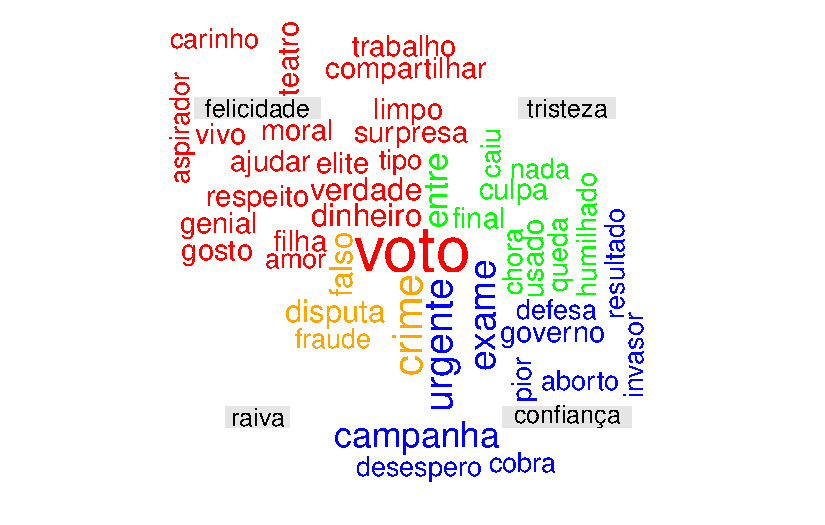
\includegraphics{boulos_files/figure-pdf/unnamed-chunk-9-1.pdf}




\end{document}
